\chapter{Návrh}

Nyní by již čtenář měl být seznámen s cílem naší práce i s nástroji, které k jeho dosažení hodláme použít. Přistupme tedy k návrhu našeho řešení.

V této kapitole nejprve čtenáři představíme objektový návrh, který bude použit při implementaci, a poté zevrubně prodiskutujeme metody zpracování uživatelského vstupu pro účely ovládání meče a hráčské postavy.


\section{Objektový návrh}

Chceme vytvořit akční hru zaměřenou na boj s mečem. Základními požadavky tedy je, aby hráč mohl chodit po herním světě, máchat svou zbraní a tím zraňovat další entity. Takovými entitami může být víceméně cokoliv - např. trénovací panák nebo nosný trám nepřátelské věže - avšak bylo by pěkné, kdybychom umožnili, aby jedním z typů nepřátel byl i počítačem řízený ekvivalent hráčské postavy.

\begin{figure}[p]\centering
    \center
    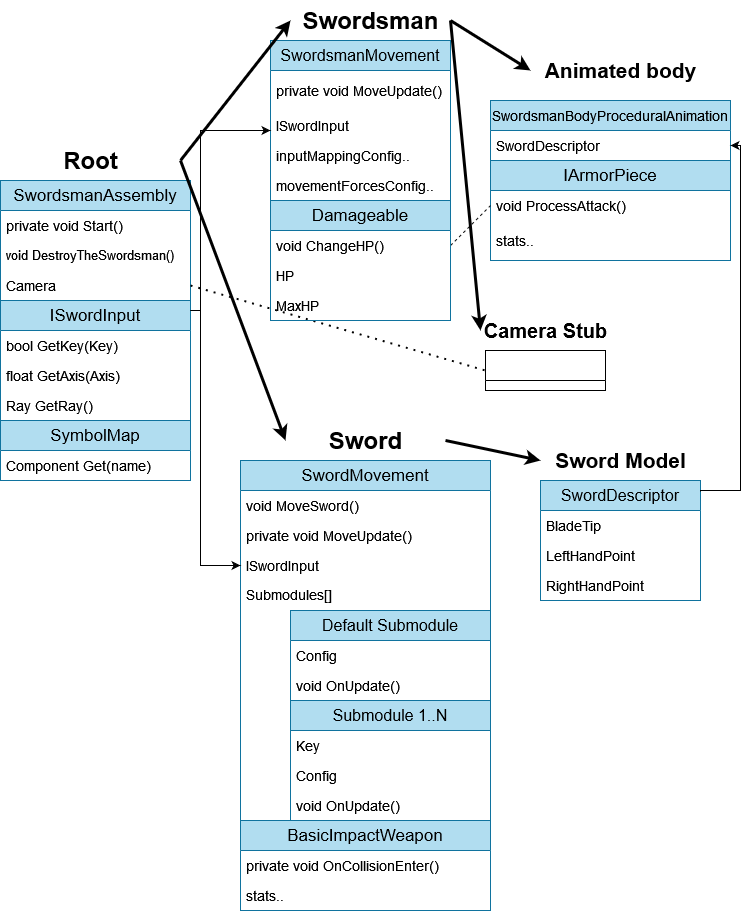
\includegraphics[width=145mm]{../img/Structure-diagram.png}
    \caption{Diagram znázorňující strukturu našeho systému}
    \label{obr04:objectModelDiagram}
\end{figure} 

\subsection{Abstrakce uživatelského vstupu}

Než se pustíme do modelování herních entit, bude vhodné nejprve vytvořit abstrakci nad zdrojem uživatelského vstupu. Jak jsme čtenáři představili v \ref{unityInputExplanationSubsection}, vstup je tradičně získáván pomocí statických metod třídy \texttt{UnityEngine.Input}. To je metoda velmi rigidní - implikuje jediný globální zdroj vstupu pro všechny objekty, nad jehož obsahem navíc nemáme žádnou kontrolu. 

Co bychom chtěli je možnost konfigurovat různé zdroje vstupu pro různé objekty - např. hráčská postava může být ovládána pomocí hodnot získaných z \texttt{UnityEngine.Input}, počítačem řízení protivníci by o nich však neměli mít ponětí. Při vhodném návrhu by mělo stačit naprogramovat a otestovat hráčského šermíře a nepřátelského z něj následně vytvořit pouhou výměnou zdroje vstupu za vstup simulovaný algoritmem umělé inteligence.

Ustanovíme tedy rozhraní \textbf{\texttt{ISwordInput}}. Jeho metody budou pro jednoduchost rámcově odpovídat vybraným základním metodám z \texttt{UnityEngine.Input}. Jeho základní implementace - komponenta \textbf{\texttt{BasicSwordInput}} bude jednoduše volat odpovídající metody \texttt{UnityEngine.Input}, avšak nic nám nebrání vytvořit libovolně mnoho variant s jinou vnitřní logikou. 

Stanovíme konvenci, že každý objekt, jenž zpracovává uživatelský vstup, si jeho zdroj při své inicializaci najde v objektové hierarchii voláním \texttt{GetComponentInParent<ISwordInput>()} (viz \ref{howToSearchForComponentsSubsubsection}).


\subsection{Šermíř}

Nyní můžeme přistoupit k návrhu základních herních entit. 

Začněme postavou šermíře. Ten je samostatným herním objektem, jehož náplní práce je pohybovat se po herním světě, držet meč a být zasahován nepřátelským mečem. Pohybovat by se měl dle instrukcí získaných z hráčského vstupu, zároveň v jeho očích sídlí kamera, skrze kterou hráč herní svět vnímá.

Zodpovědnou za pohyb hráče a kamery stanovíme komponentu \textbf{\texttt{SwordsmanMovement}}. Ta bude znát několik pevně daných způsobů pohybu - chůze dopředu/dozadu, otáčení doleva/doprava, skok apod. - pro každý z nich konfigurované mapování vstupu, rychlost pohybu apod., a dle hodnot přečtených ze své instance \texttt{ISwordInput} bude tyto pohyby vykonávat. 

Jedním z dětí šermířského objektu bude \textbf{kamera}, která se otáčí za šermířovým pohledem. Avšak uzurpovat pro sebe skutečnou herní kameru není vhodné - v případě šermířovy smrti by pak kamera rovněž byla zničena a hra by se dostala do nekonzistentního stavu. Navíc nechceme, aby kameru ovládali nepřátelští šermíři. Místo skutečné kamery tedy budeme otáčet a polohovat její maketu - poslouží prázdný objekt s komponentou \texttt{Transform} - při inicializaci šermíře volitelně na skutečnou kameru umístíme jednoduchý skript, který bude jejich pozice synchronizovat.

Dalším dítětem šermířského objektu bude šermířův detailní animovaný model. Na něm bude umístěna soustava colliderů určených ke kolizi s nepřátelskými zbraněmi. Rovněž ponese komponentu \textbf{\texttt{SwordsmanBodyProceduralAnimation}} zodpovědnou za procedurální animaci šermířových rukou - aby se kosmeticky tvářily držet meč\footnote{V ranném testováním jsme zjistili, že meč reálně držený v šermířových rukou by značně zkomplikoval náš návrh, umocnil nestabilitu fyzikální simulace a nepřinesl by nám mnoho benefitů.}.


\subsection{Meč} 

Nejdůležitějším herním objektem našeho systému je meč. Jak jsme si stanovili v kapitole \ref{goalSettingChapter}, chceme, aby byl modulárně schopen přijímat různé metody ovládání a aby rozhraní, skrze které s ním ovládací moduly komunikují, umožnilo volný pohyb ve všech 6 stupních volnosti.

\subsubsection*{Moduly} \label{interfacesSwordMovementModulesObjectModelSubsubsection}

Protože každá z metod vstupu bude vynikat v jiné situaci, bylo by velmi příhodné, kdyby mezi nimi bylo možné přepínat velmi jednoduše v žáru boje - například stisknutím klávesy. Taková schopnost má potenciál celkovou flexibilitu ovládání znásobit - např. hráč může defaultně používat ovládací mod pro sekání, ale jakmile je třeba, bleskově přepnout do specializovaného modu pro blokování, následně provést protiútok přepnutím do dalšího modu specializovaného pro bodání. 

Nabízí se tedy ovladací komponentu \textbf{\texttt{SwordMovement}} implementovat jako \textbf{stavový automat}. Jednotlivé stavy - moduly - budou zodpovědné za výpočet polohy, kam se meč má přesunout. Samotná komponenta \texttt{SwordMovement} pak modulům poskytne rozhraní, skrze které přesun na konkrétní vypočtenou polohu vyžádají, a bude zodpovídat za průběh onoho přesunu. Rovněž bude třeba držet přehled, který modul je právě aktivní, a na tom si každý snímek vyžádat aktualizaci stavu.

Jak tedy vypadá náš hotový návrh? Abstraktní třídou, ze které moduly dědí, nechť je \texttt{SwordMovement.Module}. Ta definuje množinu funkcí jako \texttt{OnActivated()}, \texttt{OnDeactivated()}, \texttt{OnFixedUpdate()}, které na modulu jsou v závislosti na jeho stavu volány - každý modul je může overridovat vlastní logikou. Na začátku hry je rovněž do každého modulu injectnuta reference na \texttt{ISwordMovement} (podmnožina celkové funkcionality \texttt{SwordMovement}), která poskytuje zdroj uživatelského vstupu, deskriptor meče, transform šermíře, který meč drží, a konečně funkci \texttt{MoveSword()}, jejímž voláním skript vyžádá změnu polohy meče.

Seznam modulů lze konfigurovat z editoru. Každá instance \texttt{SwordMovement} definuje jeden výchozí modul (aktivní když žádná klávesa není stisknuta) a list key-value párů, kde klíčem je klávesa a hodnotou modul, který se stisknutím klávesy má aktivovat. Každý typ modulu rovněž může definovat dodatečná data, která z editoru lze konfigurovat (dle klasických pravidel serializace). Není problém mít definováno na různých klávesách dva moduly stejného typu, ale s různou konfigurací.

Metoda \texttt{MoveSword()}, kterou řidicí komponenta modulům poskytuje, bere jako argument strukturu, která udává cílovou polohu, natočení meče a rovněž dodatečné volitelné parametry - např. jakou silou má meč být držen. Vlastní pohyb meče do tohoto stavu je plně v režii komponenty \texttt{SwordMovement} - ta pouze ručí za to, že pohyb bude plynule rozprostřený v průběhu času a bude se chovat standardním způsobem bez ohledu na to, s jakou četností je \texttt{MoveSword()} voláno (ať již každý \texttt{FixedUpdate} či třeba jen jednou za sekundu).

\subsubsection*{Model meče} \label{interfacesSwordModelSubsubsection}

Rovněž je třeba stručně zmínit samotný model meče. Ten zahrnuje jak mesh, který se bude vykreslovat na obrazovce, tak fyzikální collidery. V herní logice budeme potřebovat s mečem pracovat zjednodušeně jako s množinou jeho význačných bodů (špička a pata čepele, začátek a konec rukojeti apod.).

Model a collidery vytvoříme pomocí standardních komponent. Význačné body oproti tomu jsou velká množina prázdných herních objektů, se kterými pracovat jednotlivě by bylo velmi úmorné - vytvoříme tedy komponentu \textbf{\texttt{SwordDescriptor}}. Ta nechť definuje pro každý význačný bod pojmenovanou proměnnou, kam bod zkrátka přiřadíme v editoru. Do skriptů, které nad nimi operují, nyní stačí předat odkaz na tuto komponentu.


\subsection{Kořen hierarchie} 

Šermíř a meč dohromady tvoří jednu celistvou, hráčem ovladatelnou entitu. Potřebujeme tedy jeden objekt, který je bude oba zaštiťovat jako kořen prefabu a zaručí, že jsou vzájemně korektně pospojované. Obě tyto komponenty rovněž potřebují komunikovat s objekty vnějšího světa - číst uživatelský vstup, polohovat kameru, updatovat healthbar,... - bylo by tedy vhodné, aby tento kořen hierarchie posloužil i jako spojník s vnějším světem. 

Za úspěch budeme považovat, pokud veškeré změny, jenž musí proběhnout k přetvoření hráčského šermíře na počítačem řízeného protivníka, omezeníme výhradně na obsah tohoto objektu.

\subsubsection*{Vstup}

Kořen hierarchie přirozeně bude místem, kde definujeme instanci \textbf{\texttt{ISwordInput}}. Šermíř i meč ji zde - ve svém předkovi - automaticky najdou aniž bychom museli vynakládat větší úsilí.

\subsubsection*{SwordsmanAssembly}

Komponentu \textbf{\texttt{SwordsmanAssembly}} určíme zodpovědnou za pospojování šermíře a meče dohromady. Rovněž bude zodpovídat za propojení šermíře s kamerou, jejíž referenci zde volitelně nakonfigurujeme. 

\subsubsection*{SymbolMap}

Komponent uživatelského rozhraní a dalších součástí vnějšího světa je větší množství a interakce s každou z nich probíhá specifickým způsobem - tu tedy nechme plně v režii interagujícího podobjektu. Zde poskytneme pouze možnost definovat reference na ně, na ty se následně objekty uvnitř budou moci symbolicky odkazovat.

Komponenta \textbf{\texttt{SymbolMap}} poskytne z editoru konfigurovatelný list, ve kterém můžeme skladovat reference na libovolné komponenty herního světa - ke každé přiřazený string s unikátním jménem. V komponentě uvnitř šermíře či meče pak můžeme definovat serializovatelnou proměnnou typu \textbf{\texttt{Symbol}} - uživatel v editoru zadá jméno, skript pak voláním \texttt{symbol.Get()} získá příslušnou komponentu.


\subsection{Systém zranění}

Posledním dílem skládačky naší hry je hráčova schopnost zraňovat další entity a být jimi zraňován. Pro jednoduchost volíme cestu tradičního systému bodů zdraví a zranění.

Zde najdeme 3 podstatné druhy komponent - \textbf{zbraň}, která udílí zranění, \textbf{oběť útoku}, jež zranění přijímá a případně je schopna zemřít, a konkrétní \textbf{část těla}, jež byla zasažena.

\subsubsection*{Damageable}

Komponenta v kořenu postavy, která definuje její body HP - v našem případě tedy šermíř. Nabízí eventy pro situace, kdy je zraněna či léčena (aby bylo updatováno GUI apod.), v případě že HP klesnou na 0 buď může svůj herní objekt okamžitě zničit, či zavolat event, který provede zničení sofistikovaněji (např. hráče respawne). 

Změna HP se provádí voláním funkce \texttt{ChangeHP(float)} - předáváme-li kladný argument, je chápáno že jde o léčení, záporný argument znamená zranění.

\subsubsection*{Zbroj}

Zranění je typicky vyvoláno zasažením některé z částí těla postavy. Ty mohou být různě obrněné a nabízet různou míru tlumení útoku. Reprezentujeme je komponentami dědícími z \textbf{\texttt{IArmorPiece}}. V našem případě budou rozmístěny v detailím těle šermíře jako doprovod jednotlivých colliderů.

Chceme-li vykonat útok na konkrétní kus zbroje, voláme funkci \texttt{ProcessAttack(AttackDeclaration)}, kde \texttt{AttackDeclaration} je struktura nesoucí základní informace o bodu, kam byl proveden zásah, míře způsobeného zranění apod. . Instance zbroje následně přepočítá, jaké zranění bylo reálně způsobeno a zavolá \texttt{ChangeHP()} na \texttt{Damageable}, které nalezlo ve svém předkovi.

\subsubsection*{Zbraň}

Zbraň je jakýkoliv objekt, který je na \texttt{IArmorPiece} schopen volat \texttt{ProcessAttack()}. Může to být např. paprsek smrti řízený raycastem, avšak v našem případě to typicky bude fyzikální objekt, jenž deklaruje útok při kolizi s jiným objektem. 

Konkrétní implementací, kterou použijeme, je \textbf{\texttt{BasicImpactWeapon}}. Její náplň práce je zkrátka při každé zprávě \texttt{OnCollisionEnter} prozkoumat zasažený collider, zda někde v jeho předkovi není \texttt{IArmorPiece} - pokud je, vytvoří pro něj deklaraci útoku na základě bodu zásahu a síly kolize, jež mu byly nahlášeny fyzikálním systémem. 

Tuto komponentu v našem případě umístíme do kořenového objektu meče\footnote{Bylo by pěkné moci ji umístit přímo do čepele, jak jsme však zmínili v \ref{collidersPhysicsIntroSubsection}, komponenta poslouchající na \texttt{OnCollision} se musí nalézat ve stejném objektu jako \texttt{Rigidbody}.}.



\subsection{Zhodnocení návrhu} 

Skutečnou míru kvality našeho návrhu poznáme až po dlouhých letech jeho neodvratného živelného vývoje v praktickém nasazení, nyní můžeme nanejvýše prohlásit, že náš návrh se zdá být v souladu s principy \texttt{SOLID} \cite{CleanArchitectureSOLID}. 

Herní systém jsme dekomponovali do soustavy herních objektů s komponentami - základem jsou šermíř a meč, které uzavíráme do společného předka majícího úkol pospojovat je navzájem a s vnějším světěm. 

Šermíř a meč jsou samostatné entity, jejich herní logika je dobře oddělená. Datové závislosti mezi nimi existují, ale jsou read-only - šermíř zkrátka potřebuje znát aktuální polohu meče, aby jej mohl držet ve svých rukou.

Největší komplexita se bude soustředit do \textbf{ovládání meče}. Jeho logiku jsme se tedy pokusili učinit otevřenou pro rozšíření jak jen to bylo možné. Oddělili jsme low-level objekt zodpovědný za uskutečnění pohybu meče (\texttt{SwordMovement}) a high-level objekty (\texttt{SwordMovement.Module}), jež z uživatelského vstupu pro low-level objekt generují instrukce. Oba spolu komunikují přes dobře definované rozhraní a není problém přidávat nové jejich implementace či je obalovat do dekorátorů. High-level submodulů dovolujeme mít definované libovolné množství - aktivní je vždy pouze jeden, ale lze mezi nimi velmi rychle přepínat. 

Veškeré spojení s objekty vnějšího herního světa (např. GUI) jsme soustředili do \textbf{kořenového objektu}. Zde je možné libovolné vnější komponenty odkázat a vnitřní objekty je dohledají dle stanoveného identifikátoru.

Také jsme vytvořili abstrakci pro uživatelský vstup (rozhraní \texttt{ISwordInput}) - výměnou použité implementace by neměl být problém později hráčského šermíře např. změnit na počítačem řízeného nepřítele. Jeho instanci rovněž vnitřní objekty naleznou v kořenovém objektu. 

Celý náš systém jsme nakonec protkali systémem zranění. Ten je dle našeho návrhu velmi jednoduchý, ale poskytuje značnou úroveň rozšířitelnosti. Není problém, aby různé části těla postavy (oblečené do různé části zbroje) vyhodnocovaly zranění různým způsobem. Zbraní pak může být naprosto jakákoliv entita schopná na části zbroje volat metodu \texttt{ProcessAttack()}, nejsme tedy nutně omezeni pouze na zraňování působením fyzikálních sil.


%------------------------------------------------------------------------------------------------------------------------------------------------------------------------------------------------------------------------------------------------------------%
 % xxxxxxxxxxxxxxxxxxxxxxxxxxxxxxxxxxxxxxxxxxxxxxxxxxxxxxxxxxxxxxxxxxxxxxxxxxxxxxxxxxxxxxxxxxxxxxxxxxxxxxxxxxxxxxxxxxxxxxxxxxxxxxxxxxxxxxxxxxxxxxxxxxxxxxxxxxxxxxxxxxxxxxxxxxxxxxxxxxxxxxxxxxxxxxxxxxxxxxxxxxxxxxxxxxxxxxxxxxxxxxxxxxxxxxxxxxxxxxxxxxxxxxxx %
%------------------------------------------------------------------------------------------------------------------------------------------------------------------------------------------------------------------------------------------------------------%



\section{Schéma ovládání} 

Rozhraní, skrze která budou jednotlivé komponenty herního systému komunikovat mezi sebou, již máme. Nyní se zaměřme na rozhraní, skrze které s nimi bude komunikovat uživatel.

Tomu potřebujeme především poskytnout kontrolu nad pohybem jeho postavy v herním světě a nad pohybem meče, který postava drží.

Jak jsme se rozhodli v kapitole \ref{goalSettingChapter}, chceme, aby naše hra byla přístupná pro běžného uživatele, který je vybaven pouze myší a klávesnicí.

\subsection{Ovládání meče - úvodní zamyšlení}

Jak jsme již na mnoha místech nastínili, ovládání meče je v naší situaci těžkým problémem, začněme tedy tím. 

\subsubsection*{Rozbor možností}

Víme, že plnou kontrolu ve všech šesti stupních volnosti hráči poskytnout nemůžeme. Nezbývá nám než z této celkové množiny stavů vybrat nějakou podmnožinu, na kterou jsme schopni vstup z myši a klávesnice namapovat.

Mapování musí především pro hráče být jednoduše myšlenkově uchopitelné. Zároveň ho nechceme omezit na konečnou množinu stavů. Potřebujeme tedy nalézt vhodný matematický formalizmus pro jeho popis - ideálně nějaký, který se bude chovat spojitě\footnote{Spojitost neformálně definujme např. takto: Pro každé dvě polohy kurzoru \texttt{A}, \texttt{B} a mapování \texttt{f}, pokud \texttt{C} je poloha kurzoru nacházející se na cestě z \texttt{A} do \texttt{B}, pak poloha meče \texttt{f(C)} je stejným způsobem mezistav pro \texttt{f(A)}, \texttt{f(B)}.} a budeme schopni ho pro hráče přehledně vizualizovat. 
\bigbreak
Hra \textbf{\acl{DbtS}} (viz \ref{dieByTheSwordDescriptionSubsection}) řešila velmi podobný problém jako my. Podívejme se tedy nejprve na metody, které svým hráčům poskytla:
\begin{itemize}
    \item \textbf{Numerická klávesnice} - Existovala pouze pro zajištění přístupnosti v době, kdy myš nebyla rozšířená. Umožňovala malou podmnožinu toho co myš a nijak při tom nezvyšovala uživatelskou přívětivost.
    \item \textbf{Myš} - Jediný z ovladačů, který poskytl spojité mapování. Vyžadovala cvik, ale umožnila kreativní a flexibilní reakce v neočekávané situaci.
    \item \textbf{Nahrávky} - Technicky s mečem umožnily vykonávat libovolné pohyby, těchto pohybů však v libovolném okamžiku muselo být definováno malé konečné množství. Hráč tedy nebyl schopen flexibilně reagovat na specifickou situaci. 
\end{itemize}
Z tohoto náhledu je zřejmé, že všechny metody kromě myši z podstaty věci smrsknou množinu stavů na konečné množství a neumožní rychlé flexibilní reakce. Dále se tedy zaměříme primárně na použití myši. Klávesnice může zastávat konečné množství doplňujících funkcí, které se na myš nevešly. Nahrávky bude rovněž vhodné interně implementovat, aby byly v případě potřeby k dispozici pro počítačem řízeného nepřítele (v jeho případě je předvídatelnost a nízká flexibilita výhodou).
\bigbreak
\textit{Není možné vyloučit, že existují neznámé alternatní způsoby využití myši a klávesnice, které se vymykají závěrům tohoto našeho zamyšlení. Jejich prozkoumání však ponecháme případným navazujícím pracím. Pro ty zde vytvoříme jednoduše myšlenkově uchopitelný kontrolní bod, proti kterému budou moci své výsledky experimentálně srovnávat.}

\subsubsection*{Volba mapování}

Nástroj ovládání máme stanovený, jaký se tedy nabízí formalizmus pro mapování kurzoru na polohu meče?

\acl{DbtS} umožňuje hráči velmi dobře sekat mečem. Jakým přesným způsobem mapování vykonává, to však není možné bez přístupu ke zdrojovému kódu zjistit. Pokusme se nyní vlastní cestou dobrat k podobnému výsledku.

Po krátkém zamyšlení nad metodami, které nám pro zpracování dat z myši poskytuje Unity (viz \ref{unityInputExplanationSubsection}), jsme se rozhodli, že dobrým krokem pravděpodobně bude vystřelit z pozice kurzoru paprsek do herního světa. Tento paprsek bychom následně mohli protnout skrze nějaký jednoduchý geometrický útvar, který jsme schopni hráči dobře vizualizovat. 

Kdybychom pro jednoduchost prohlásili, že poloha rukojeti meče je nehybná, získaný průnik můžeme interpretovat jako pozici, kam má čepel meče směřovat. Pohybem kurzoru plynule zleva doprava by pak meč měl vykonat sek - rovněž zleva doprava. Plynulost a finesa, s jakými sek bude proveden, závisí na útvaru, který protínáme. 

Po kratší úvaze jsme se rozhodli, že útvarem, se kterým se pokusíme paprsek protínat, je \textbf{kulová plocha}. Nabízí nám plynulý přechod mezi stavy, jak se kurzor pohybuje po obrazovce, a její vizualizace nečiní problém (viz obr.\ref{obr04:sphereVisualization}).
\bigbreak
Provedeme tedy experimentální implementaci s její pomocí, tu otestujeme, a v případě potřeby ji použijeme jako výchozí bod pro implementaci sofistikovanějšího systému.

\begin{figure}[ht]\centering
    \center
    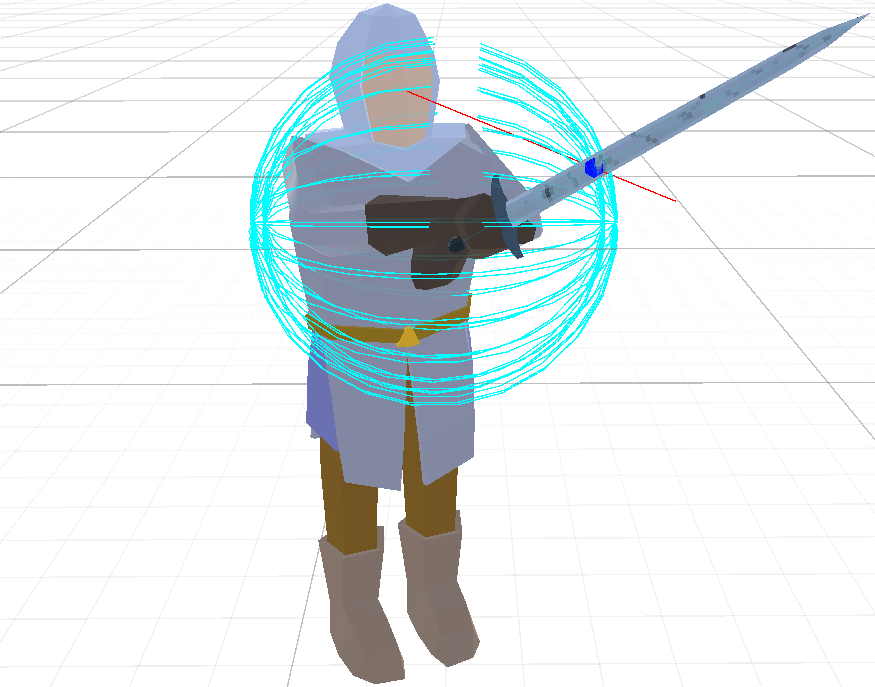
\includegraphics[height=90mm]{../img/IntersectableSphere.png}
    \caption{Vizualizace - Ovládání meče průnikem paprsku s kulovou plochou}
    \label{obr04:sphereVisualization}
\end{figure} 

\pagebreak

\subsection{Ovládání meče - moduly} \label{interfacesSwordMovementModulesSubsection}

Nyní tedy náš systém dovoluje sekat mečem podobně dobře jako \acl{DbtS}. Sekání však zdaleka není jediný typ úkonu, který s mečem má smysl vykonávat. Je tedy nějaký způsob, jak náš současný návrh zobecnit, aby podporoval i další typy pohybu?

Jedním možným řešením je představit další mody ovládání, specializované na specifické činnosti, podobně jako ten náš současný je na sekání. Přepínání mezi nimi nebude jakkoliv záviset na poloze kurzoru - tím by možnosti každého jednotlivého modu utrpěly. Naopak, zde přichází ke slovu klávesnice. Hráči zkrátka dáme možnost ke každému modu přiřadit jednu klávesu - dokud ji hráč drží, tak je daný mod aktivní, jinak se používá ten, který hráč nastavil jako výchozí.

Mapování jednotlivých poloh meče pomocí průniku paprsku a kulové plochy ponecháme jak je, pouze přidáme vrstvu abstrakce - výsledný průnik zkrátka poskytneme aktuálně aktivnímu modu ovládání jako vstup, na základě kterého má polohu meče určit. Zda ho interpretuje jako bod, do kterého směřuje čepel meče ukotveného v pevném bodě či jakkoliv jinak, je plně v jeho režii.

Pro účely naší práce jsme takové mody implementovali dva - pro sekání (který jsme nastínili výše) a pro blokování. Ty si nyní blíže popíšeme.

\subsubsection*{Formát příkazů pro meč}

Než přistoupíme k popisu, nejprve stručně nastíníme formát, jímž je poloha meče udávána. Důvody, proč byl zvolen, ponecháme sekci \ref{swordMovementMoveSwordImplementationSubsection} v implementační kapitole.

Polohu meče definujeme těmito třemi vektory:
\begin{enumerate}
    \item \texttt{Poloha rukojeti} - Meč je šermířem držen v jediném bodě, jenž se nachází uprostřed jeho rukojeti. Zde poskytnutý bod udává polohu relativní vůči šermíři, kde se tento střed rukojeti má nalézat.
    \item \texttt{Směr meče} - Směr udávající natočení meče v prostoru kolem středu jeho rukojeti. Pokud přičteme vektor Směru natočení k Poloze rukojeti, dostaneme bod, kterým by čepel meče měla procházet.
    \item \texttt{Normála na čepel meče} - Směr natočení sám nestačí na plné určení rotace meče se všemi 3 stupni volnosti - nedá nám informaci ohledně rotace kolem jeho vlastní osy (natočení čepele). Tento směr by měl být ortogonální na Směr natočení. Obě hrany ostří čepele se budou nalézat v rovině určené Bodem rukojeti a touto normálou.   
\end{enumerate}

\begin{figure}[ht]\centering
    \center
    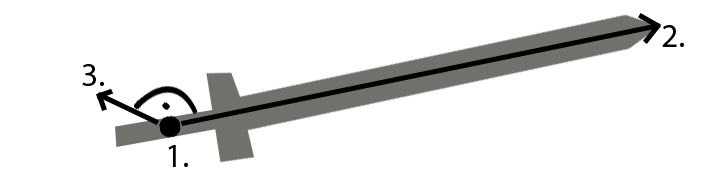
\includegraphics[width=140mm]{../img/diagram-swordPositioning.png}
    \caption{Diagram znázorňující kontrolní body meče}
    \label{obr04:swordPositioningDiagram}
\end{figure} 


\subsubsection*{Mod pro sekání}

Mod pro sekání jsme si již výše letmo nastínili, nyní ho popišme řádně. Jeho logika je velmi jednoduchá.

Na vstupu dostane tyto informace:
\begin{enumerate}
    \item \texttt{Bod průniku} - Bod ve kterém paprsek protnul ovladací kulovou plochu
    \item \texttt{Minulý Směr meče} - Směr meče zapamatovaný z hlášení předchozího snímku
    \item \texttt{Bod rukojeti} - Pevně určený bod\footnote{Po představení \texttt{IRayIntersectables} v další sekci je z konstantního bodu změněn na bod určený nahlášeným středem protunutého útvaru (viz \ref{resultSwordControlsSolutionSubsubsection}).}
\end{enumerate}

Algoritmus probíhá takto:
\begin{enumerate}
    \addtocounter{enumi}{-1}
    \item Pokud k žádnému průniku nedošlo, algoritmus skončí a meči ponechá jeho dosavadní cílovou pozici. Jinak pokračuje.
    \item Jako hodnota \texttt{Polohy rukojeti} je zkrátka nahlášen \texttt{Bod rukojeti}, získaný ze vstupu.
    \item \texttt{Směr meče} je stanoven jako vektor směru vedoucího z \texttt{Bodu průniku} do \texttt{Bodu rukojeti} - čepel zkrátka prochází \texttt{Bodem průniku}.
    \item \texttt{Normála na čepel meče} je určena jako vektorový součin \texttt{Současného} a \texttt{Minulého směru meče}. Ostrá hrana čepele je tedy natočena tím směrem, kam se meč v průběhu času pohybuje. 
    \item Nakonec algoritmus předá vypočítané instrukce meči a nastaví hodnotu Minulého bodu průniku pro použití v příští iteraci.
\end{enumerate}

\begin{figure}[ht]\centering
    \center
    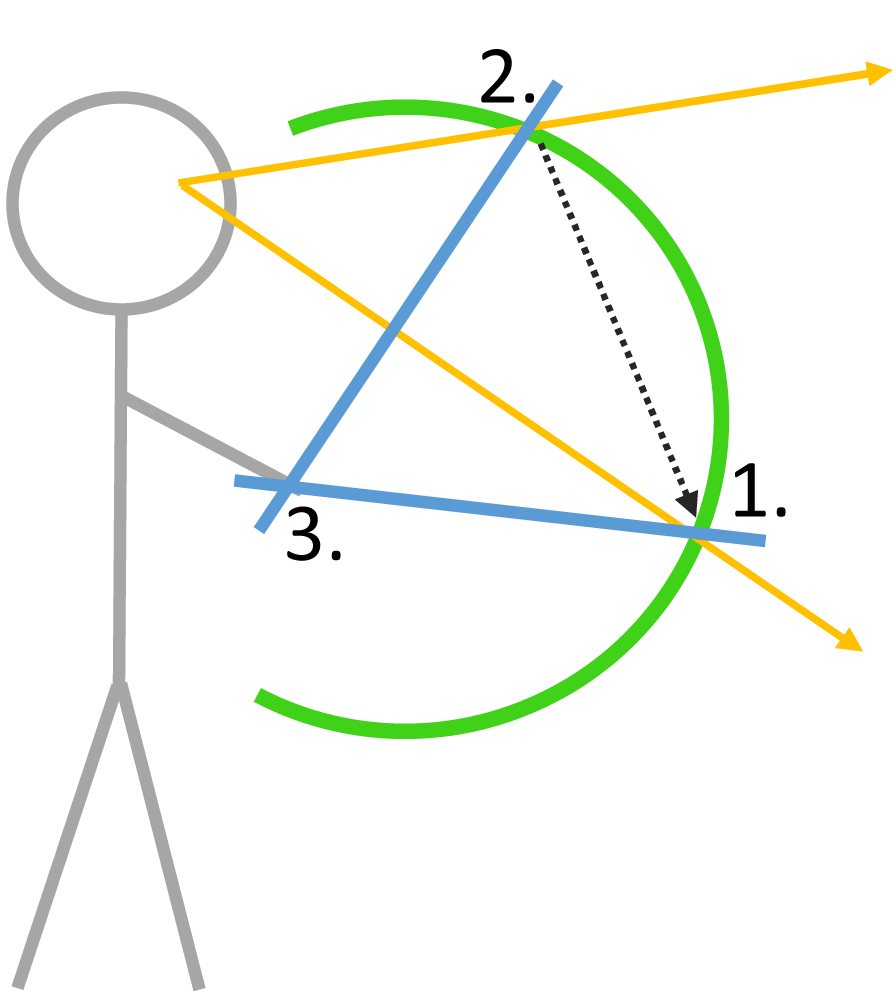
\includegraphics[width=60mm]{../img/diagram-slashingMode.png}
    \caption{Náčrt znázorňující mod sekání zjednodušeně ve 2D (meč modře, paprsek žlutě, kulová plocha zeleně, vstupní body znázorněny dle číslování výše)}
    \label{obr04:swordSlashingMode2D}
\end{figure} 
 
Výsledkem je meč, který šermíř drží v jednom bodě\footnote{To není problém - nic nám nebrání umístit bod, ve kterém ho šermíř drží, např. do volného prostoru pod mečem, čímž dosáhneme vizuálního dojmu, že šermíř mečem mává plnohodnotně.} bodě a hráč má plnou svobodu jak s ním máchat. Čepel meče se natáčí automaticky tak, aby mířila ostrou hranou tam, kam šermíř seká.

\subsubsection*{Mod pro blokování} \label{interfacesSwordMovementBlockingModuleSubsubsection}

Mod pro blokování je o poznání složitější.

Pro jeho pochopení si nejprve zmiňme, jak blokování probíhá v reálném světě. Základní myšlenkou šermíře, na kterého je veden úder, je postavit protivníkově zbrani do cesty tu jeho tak, aby úder zastavila a nebyla náporem sražena na stranu. To znamená, že zbraň chce trefit ostrou hranou vlastní čepele\footnote{Plochá strana není praktická z mnoha důvodů - šermíř by musel zdlouhavě přehmatávat, aby meč o 90° zrotoval a měl v úchopu sílu. Meč by i tak bylo jednodušší srazit na stranu, protože plochá strana nesoustředí sílu srovantelně dobře jako tenká hrana. Dále by se tím znehodnotila ochrana rukou, kterou šermířovi poskytuje záštita.}. Bod, ve kterém nepřítelovu zbraň trefí, by rovněž měl být co nejblíže rukojeti - čím dále od ní, tím větší páka nepříteli pomáhá meč srazit na stranu.

\pagebreak

Nyní k implementaci. Na vstupu dostaneme tyto informace:
\begin{enumerate}
    \item \texttt{Bod průniku} - Bod ve kterém paprsek protnul ovladací kulovou plochu
    \item \texttt{Střed ovladací kružnice} - Střed kružnice, jíž paprsek protnul
    \item \texttt{Bod nápovědy} - Pevný bod, který nám pomůže vybrat směr meče (jeho umístění zmíníme později)
\end{enumerate}

Dále pevné body, které vyznačíme na meči:
\begin{enumerate}
    \item \texttt{Špička čepele} - Bod na meči vyznačující špičku jeho čepele, leží na středové ose meče
    \item \texttt{Bod rukojeti} - Bod, ve kterém je meč ukotven k šermířovi, leží na středové ose meče
    \item \texttt{Blokovací bod} - Bod na čepeli meče blízko u rukojeti - ten, do kterého chceme trefit nepřátelský zásah 
\end{enumerate}

Naším záměrem je napolohovat meč tak, aby optimálně vyblokoval úder vedený na \textit{Bod průniku}. Tedy aby \textit{Bod průniku} se shodoval s \textit{Blokovacím bodem} a čepel byla natočená tak, že \textit{Blokovací bod} směřuje ven od šermířova těla, odkud je pravděpodobně veden útočníkův úder. Pozic, které toto splňují, existuje nekonečně mnoho - volíme tu jednu, kde špička čepele směřuje směrem k \textit{Bodu nápovědy}.

Algoritmus, který jsme zvolili, vypadá následovně:
\begin{code}
 if(Vstup == None) return; //žádný průnik

 OsaMeče := nová Přímka(BodRukojeti, ŠpičkaČepele);

 BlokovacíBodNaOse := OsaMeče::Projekce(BlokovacíBod);

 VzdálenostBlokovacíhoBoduOdRukojeti := 
    BlokovacíBodNaOse::Vzdálenost(BodRukojeti);


 TečnáRovina := nová Rovina(
    bod: BodPrůniku, 
    normála: (BodPrůniku - StředOvladacíKružnice) 
 );
 BodKamSměřujeČepel := TečnáRovina::Projekce(BodNápovědy);


 Výstup.SměrMeče := BodKamSměřujeČepel - BodPrůniku;

 Výstup.PolohaRukojeti :=
   BodPrůniku - Výstup.SměrMeče::Normalizovaný()
   * VzdálenostBlokovacíhoBoduOdRukojeti;
  
 Výstup.NormálaNaČepelMeče := 
   TečnáRovina.Normála::VektorovýSoučin(Výstup.SměrMeče);
\end{code}


\textit{Abychom zachovali předsevzetí, že \textit{Blokovací bod} leží přesně v \textit{Bodu průniku}, měli bychom ještě \textit{Polohu rukojeti} posunout o \textit{TečnáPlocha.Normála * BlokovacíBod::Vzdálenost(BlokovacíBodNaOse)}. V praxi je to však velmi drobný detail, který opomíjíme.}

Vhodným umístěním pro \texttt{Bod nápovědy} je např. několik metrů před šermířem, ve výšce mírně nad jeho hlavou - při blokování v horní polovině šermířova těla pak meč má náklon tak akorát, aby se pohodlně blokovaly údery vedené šikmo, seshora i z boku - viz obr. \ref{obr04:blockingGood}. Spodní polovina těla tím však trpí - meč je téměř zcela vertikální a šermíř ho drží velmi nepřirozeně vypadajícím způsobem - viz obr. \ref{obr04:blockingBad}. 
 
V praxi tedy místo jediného \texttt{Bodu nápovědy} definujeme jejich množinu - použije se ten s nejmenší vzdáleností k \texttt{Bodu průniku}. Prvky množiny může být např. onen bod před šermířem mírně nad hlavou a druhý analogický bod před šermířem v úrovni jeho nohou.  

\begin{figure}[ht]\centering
    \center
    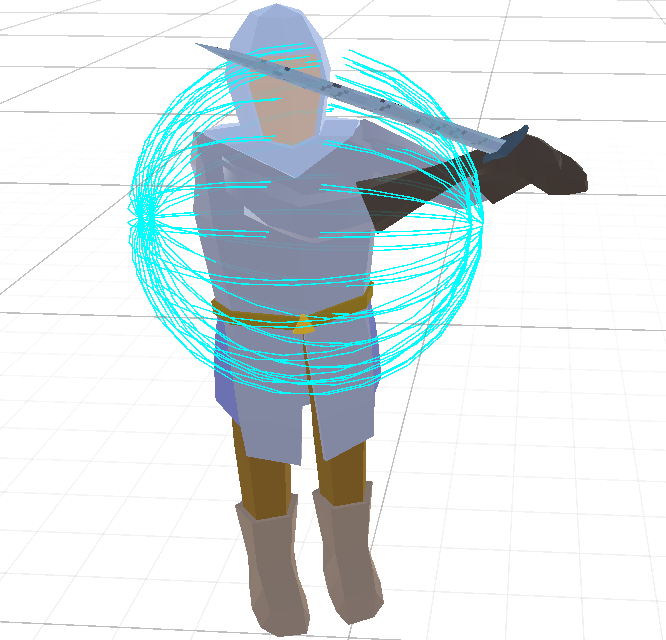
\includegraphics[height=60mm]{../img/blocking-good.png}
    \caption{Blokování v horní části těla}
    \label{obr04:blockingGood}
\end{figure} 

\begin{figure}[ht]\centering
    \center
    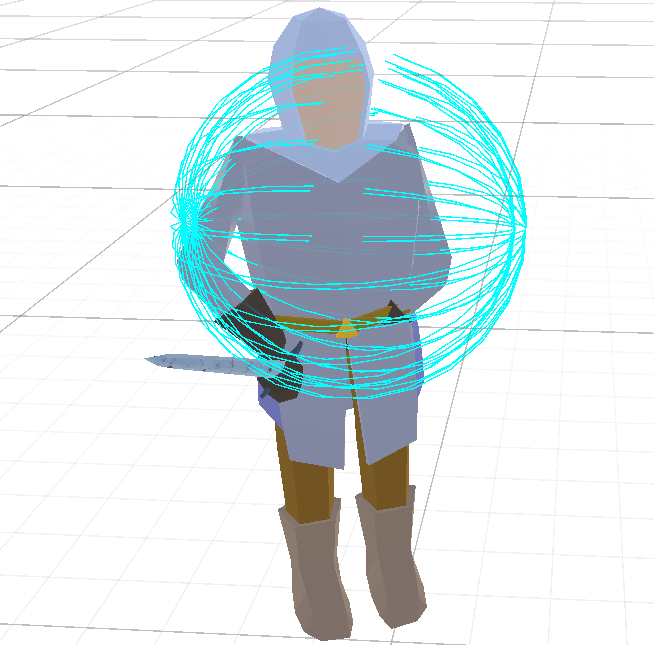
\includegraphics[height=60mm]{../img/blocking-bad.png}
    \caption{Rozbité blokování ve spodní části těla}
    \label{obr04:blockingBad}
\end{figure} 


\bigbreak

Po těchto drobných úpravách algoritmu a ručním vyladění bodů nápovědy (a průsečíkového útvaru, který představíme vzápětí) získáváme mod, s kterým lze blokovat údery vedené z široké škály směrů. Jakmile hráč získá trochu cviku, je navíc ovládání vcelku intuitivní.

\subsection{Ovládání meče - výsledek} \label{rayIntersectablesDefinitionSubsection}

Ovládání založené na kulové ploše jsme implementovali. Jak pro mod sekání, tak pro mod blokování vedlo v typickém případě k plynulému a intuitivnímu dojmu z ovládání. Narazili jsme však na některé nežádané situace v okrajových případech. Na okrajích hráčova zorného pole, kde se bod průniku nalézal v zadní polokouli kulové plochy, bylo např. velmi jednoduché, aby hráč probodl mečem sám sebe. Dalším problémem byly situace, kdy pro paprsek a kulovou plochu žádný průnik neexistoval - v takovém případě jsme neměli jako meči rozkázat změnu polohy - hráč tedy při takových polohách kurzoru nedostal od hry žádnou zpětnou vazbu, čímž utrpěl jeho pocit kontroly a ponoření do hry.

Potřebujeme tedy najít nějaké zobecnění, které zachová veškeré pěkné vlastnosti originální metody v typickém případě, ale dovolí nám podchytit veškeré nevhodné případy okrajové.

Pro vyřešení tohoto problému jsme strávili dlouhý čas živelným experimentováním. Takto vypadá výsledek, ke kterému jsme se dobrali:

\subsubsection*{Řešení} \label{resultSwordControlsSolutionSubsubsection}

Nejprve jsme stanovili rozhraní\footnote{Ve skutečnosti jde o abstraktní třídu dědící z \texttt{UnityEngine.MonoBehavior} abychom zajistili její kompatibilitu se serializačním systémem.} \textbf{\texttt{IRayIntersectable}}. To definuje jedinou metodu \texttt{GetIntersection()}, která jako argument bere paprsek a vrací strukturu popisující výsledek průniku. Tento výsledek zahrnuje flag zda byl průnik nalezen, bod průniku, střed protnutého útvaru a hodnotu určující jeho váhu.
\bigbreak
Než se dobereme k implementaci kulové plochy odpovídající tomuto rozhraní, uveďme onen nový prvek, který našemu systému razantně zvýší obecnost. Tím je \textbf{\texttt{RayIntersectableInterpolation}}. Jde o jednoduchou komponentu, která v sobě nese list odkazů na jiné \texttt{IRayIntersectables}. Jeho metoda \texttt{GetIntersection()} se chová tak, že zkrátka vyžádá průniky od všech těchto podprvků a vypočte jejich vážený průměr (dle vah získaných z návratových hodnot) - průměruje jak body průniku, tak i nahlášené středy protnutých útvarů apod. .
\bigbreak
Nyní můžeme přistoupit k \textbf{\texttt{RayIntersectableSphere}}. To je naše již známá kulová plocha, definovaná středem a poloměrem. Avšak aby ji bylo možné hladce interpolovat s vícero dalšími, přidali jsme několik dodatečných parametrů.

Nejdůležitějším z nich je \textbf{\texttt{díra}}. To je odkaz na jinou \texttt{RayIntersectableSphere}, ze které použijeme její střed a poloměr. Uvažujeme kouli jejich prostřednictvím definovanou. Myšlenka je pro každý bod průniku, který by naše koule poskytnula, se nejprve podívat na jeho vzdálenost od středu díry - pokud je průnik uvnitř díry (vzdálenost je menší než poloměr díry), průnik zahodíme, jako by k němu vůbec nedošlo. Pomocí tohoto hacku jsme schopni z konkrétní kulové plochy odebrat kus, který nám překáží - např. zadní polokouli - a zajistit tím předvídatelnější výsledek interpolace.

Nakonec jsme díru zobecnili ještě více - místo striktního je/není v díře uvažujeme poměr mezi vzdáleností bodu průniku od středu díry a jejím poloměrem (tedy číslo v intervalu \texttt{[0;1]} pokud bod leží v díře, větší než \texttt{1} pokud v díře neleží) - tuto hodnotu použijeme jako argument pro vyhodnocení uživatelsky konfigurovatelné 1D interpolační křivky\footnote{Třída \texttt{AnimationCurve} vestavěná v Unity}, její výsledek následně stanovíme jako váhu průniku. Tato varianta umožňuje vše co ta předchozí (stačí dodat křivku s hodnotou \texttt{0} v intervalu \texttt{[0;1]} a hodnotou \texttt{1} pro zbytek), avšak nově jsme schopni unvitř složité soustavy kulových ploch zajistit na hranicích mezi jednotlivými prvky plynulé přechody - váha jedné plochy pozvolna upadá zatímco váha té druhé pozvolna stoupá.

Dalším volitelnám parametrem je \textbf{\texttt{falešný střed}} - pokud ten nastavíme, výpočet průniku se nijak neovlivní, v návratové hodnotě však místo skutečného středu kulové plochy bude udána poloha tohoto bodu. Střed kružnice slouží v některých modech ovládání jako dodatečný orientační bod. Díky tomuto parametru jsme schopni složit dohromady kružnice s velmi se lišícími velikostmi a zajistit, aby se všechny tvářily jako pouhá součást jednoho celkového útvaru. 


\subsubsection*{Zhodnocení}

Slabší stránkou řešení, které jsme si právě představili, jsou možnosti jeho \textbf{vizualizace}. Jedinou cestou, kterou nám rozhraní \texttt{IRayIntersectable} umožňuje, je vyslat velké množství paprsků a vytvořit mesh pospojováním nalezených průsečíků. Taková metoda je výpočetně náročná, uživatel musí činit kompromis mezi mírou detailu a schopností běžet v reálném čase. Toto činí problém především při editaci složitějšího \texttt{IRayIntersectable} systému, kdy je značná míra detailu třeba, aby bylo možné pohledem rozpoznat, zda jsou přechody mezi sférami vlivu jednotlivých dílčích prvků plynulé. 

Přes toto drobné nepohodlí však tato metoda stále nabízí velmi mocný nástroj. Poskytnout hráči útvar, který se chová podobně intuitivně jako obyčejná kulová plocha, ale nežádané okrajové případy jsou v něm ošetřené, není obtížné - na obr.\ref{obr04:IRayIntersectableVisualization} může čtenář najít vizualizaci objektu, který hra v praxi používá pro mod blokování. 


Vynaložením většího úsilí lze vytvořit i značně komplexní útvary, jež se stále chovají plynule a spojitě\footnote{K zaručení plynulosti a spojitosti je však třeba jisté množství ruční práce při polohovaní děr a ladění jejich přechodových křivek.}. Ještě větší flexibilitu přirozeně zajišťuje možnost definice vlastních \texttt{IRayIntersectable} komponent. 

Přesto je však nutné zdůraznit, že tato konkrétní metoda vznikla jako produkt živelného experimentování - pro navazující výzkum by pravděpodobně nemělo být obtížné nalézt alternativu, která tvůrci hry poskytne stejnou moc, ale čistší a na použití pohodlnější cestou. 

 
\begin{figure}[p]\centering
    \center
    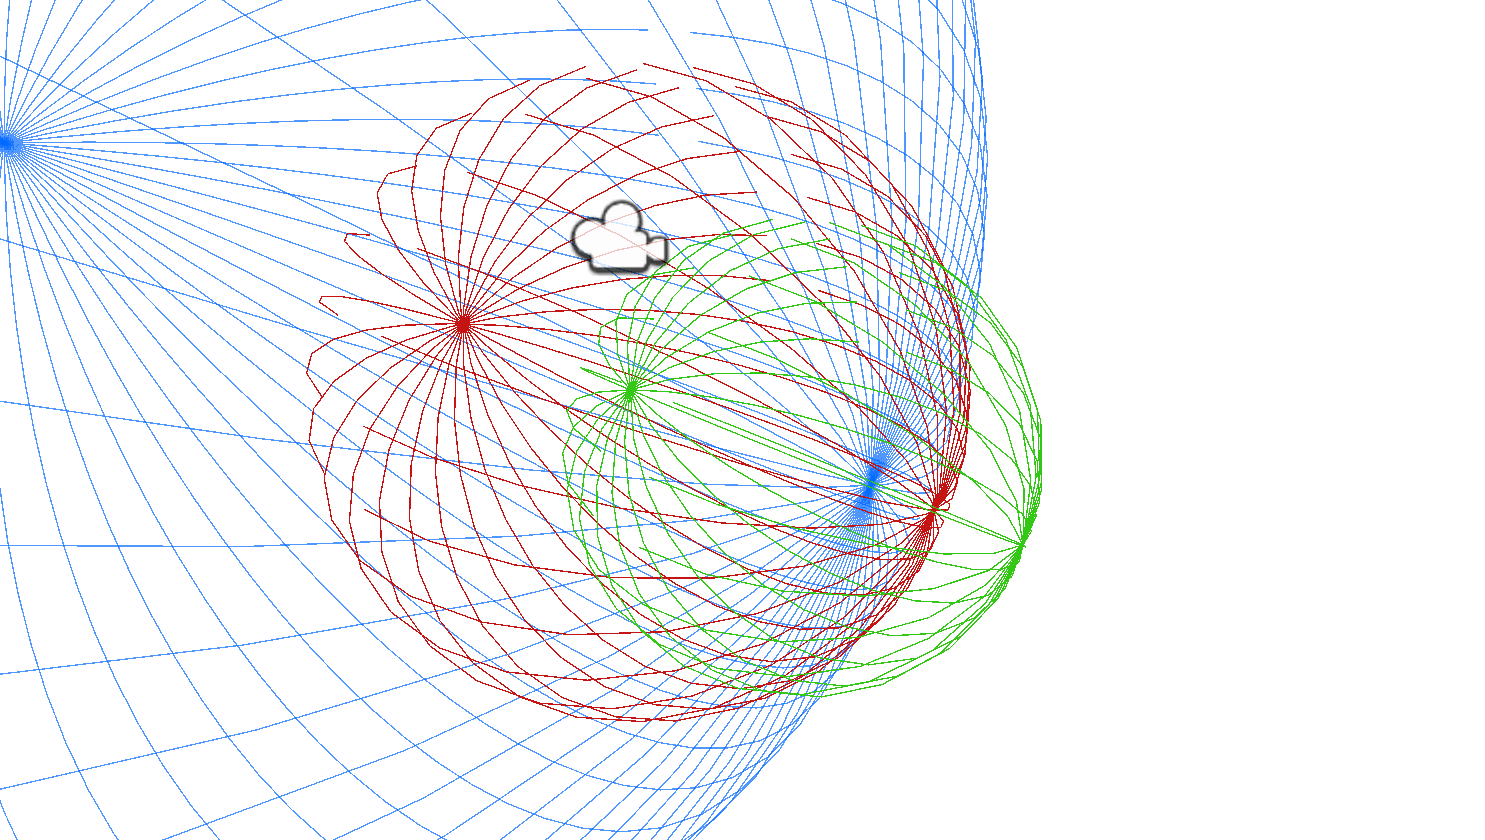
\includegraphics[width=135mm]{../img/IRayIntersectable-spheres.png}
    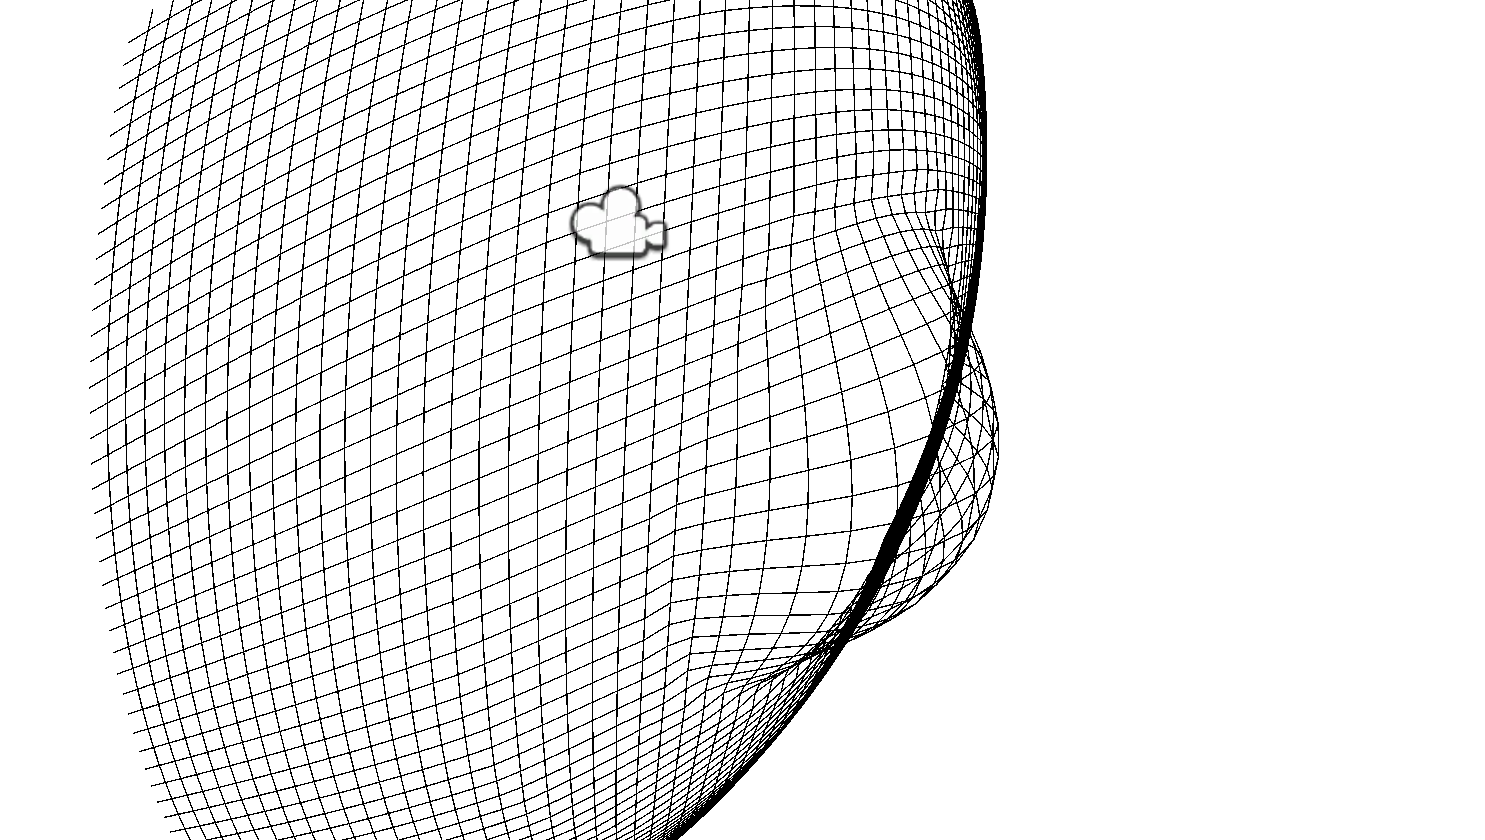
\includegraphics[width=135mm]{../img/IRayIntersectable-result.png}
    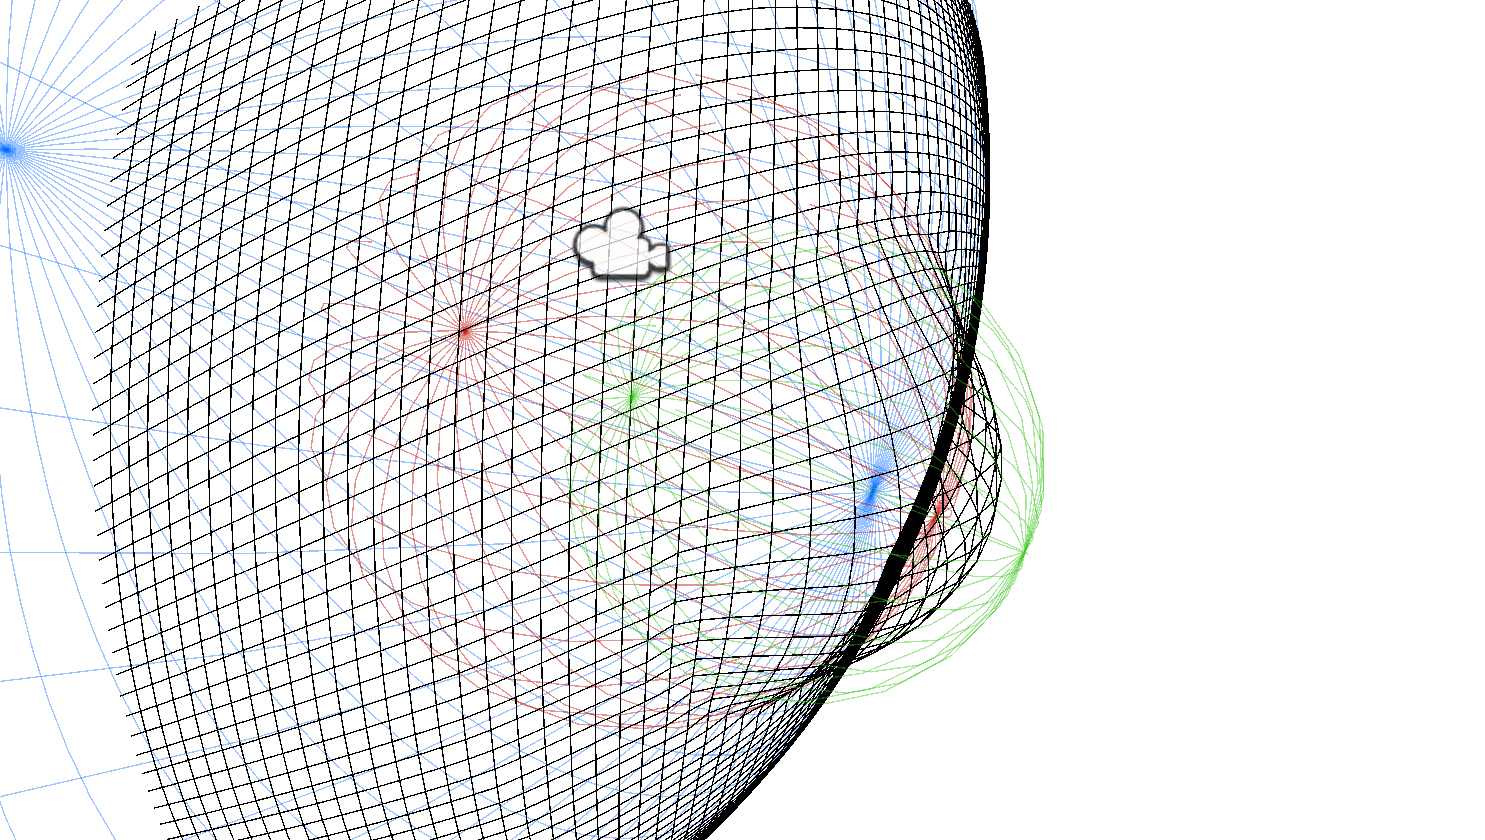
\includegraphics[width=135mm]{../img/IRayIntersectable-both.png}
    \caption{Vizualizace - složený IRayIntersectable útvar (červená koule je díra, ostatní barvy jsou dílčí prvky)}
    \label{obr04:IRayIntersectableVisualization}
\end{figure} 

\pagebreak

\subsection{Ovládání postavy}

Ovládání meče tedy máme vyřešené, nyní zbývá navrhnout ovládání pohybu postavy po herním světě - ideálně takové, aby jeho zapojením ovládání meče nijak neutrpělo. 

Jako základ jsme použili klasické, všeobecně známé schéma kláves \textbf{WASD} pro chůzi dopředu, dozadu a úkroky do stran. Ovládání meče z takového rozhodnutí nijak netrpí, naopak se tím levá ruka dostává do oblasti klávesnice, kde se nalézá mnoho kláves (Shift, Ctrl,...) přirozeně se nabízejících pro přepínání mezi jednotlivými mody ovládání meče.

Problémem je však \textbf{rozhlížení} hráčské postavy - to bývá tradičně ovládáno pohybem myši, v naší hře je však myš plně využita pro ovládání meče - koncept, jež je k rozhlížení postavy ortogonální. 

Rozhlížení nahoru/dolů je čistě kosmetická záležitost implementovaná natáčením kamery. Po testování jsme došli k závěru, že jeho ovládání pomocí myši nemá na hráčský zážitek natolik negativní vliv, aby bylo neakceptovatelné. 

Problémem je však rozhlížení do stran - při testování vyšlo najevo, že jeho namapováním na pohyb myši vedlo k velmi matoucímu hernímu zážitku. Zvolili jsme tedy jednoduché náhradní řešení namapovat jej na klávesy QE. Toto řešení není zcela intuitivní a vyžaduje čas, aby si na něj hráč zvykl, avšak poté se zdá být použitelné poměrně dobře.

\bigbreak
Celkově jsme tedy pro ovládání postavy použili klasické schéma WASD udávající pohyb dopředu a do stran doplněné klávesami QE pro natáčení postavy do stran, myš slouží k rozhlížení pouze nahoru/dolů. Toto řešení se zdá být pro zaručení ovladatelnosti a dobrého hráčského zážitku dostatečné. Nalezení ještě lepší alternativy ponecháme jako téma pro navazující práce.

\section{Shrnutí}

V první části kapitoly jsme stanovili objektový návrh hlavních prvků našeho systému - šermíře a jeho meče. 

\textbf{Šermíř} je typickou herní postavou, která čte vstupy od uživatele a v závislosti na nich se pohybuje po herním světě (komponenta SwordsmanMovement). Je vybaven jednoduchým colliderem pro kolize s herním světem a detailním modelem, který koliduje s nepřátelskými meči a je procedurálně animován, aby se vizuálně tvářil držet vlastní meč (komponenta SwordsmanBodyProceduralAnimation). 

\textbf{Meč} je samostatným objektem v hierarchii. Drží si referenci na šermíře, jímž je držen, a při určování svého pohybu bere v úvahu jeho pozici. Celkově však probíhá pohyb meče plně v jeho vlastní režii - zodpovědnou komponentou je SwordMovement. Ta operuje jako stavový automat. Tvůrce hry v editoru nakonfiguruje seznam stavů (potomci třídy SwordMovement.Module) a jejich mapování na stisknuté klávesy, SwordMovement pak dle vstupu od uživatele vybírá, který stav je aktivní - na tom jediném volá metodu OnFixedUpdate. V této metodě submodul provádí libovolnou vnitřní logiku (konkrétní příklady - modul pro sekání a pro blokování - jsme navrhli v 2. polovině kapitoly) a nakonec na instanci SwordMovement zavolá metodu MoveSword(), které jako argument předá žádanou pozici meče. SwordMovement se následně postará o jeho plynulý přesun. 

Meč i šermíř jsou dětmi společného \textbf{kořenového objektu} - jeho starostí je, aby byly meč a šermíř řádně pospojované jeden s druhým a s objekty vnějšího světa. Konfigurujeme zde např. zdroj uživatelského vstupu (komponenta dědící z \textbf{ISwordInput}) či reference na kameru a prvky GUI (healthbar apod.).

Celkově by tento návrh měl poskytovat dobrou rozšiřitelnost logiky pro ovládání meče (stačí přidat nový SwordMovement.Module), implementace počítačem řízených šermířů by tomuto návrhu rovněž neměla činit problém (stačí vyměnit zdroj vstupu a odebrat reference na GUI).

Tímto návrhem jsme následně protkali \textbf{systém životů a poškození} - šermíř definuje komponentu \textbf{Damageable}, jednotlivé collidery v jeho detailním těle jsou doplněny komponentami implementujícími \textbf{IArmorPiece}, schopnost je zranit je dodána meči komponentou \textbf{BasicImpactWeapon}. Systém poškození jsme navrhli velmi jednoduchý, ale rovněž značně flexibilní - není problém definovat různě se chovající zbroj pro různé části šermířova těla; zbraní je cokoliv, co je na instanci IArmorPiece schopné volat metodu ProcessAttack() - jsou tedy umožněny i typy zbraní nezaložené na fyzice.

\bigbreak

Druhou část kapitoly jsme věnovali zamyšlení nad rozhraním, skrze které bude probíhat komunikace mezi hrou a hráčem - předně jsme se zaměřili na ovládání meče (které, jak jsme nastínili v \ref{gamesWithMoreDirectControll}, představuje těžký problém).

Rozhodli jsme se pro \textbf{ovládání pomocí myši}. Nejprve jsme zkusili provádět mapování tak, že jsme dle polohy kurzoru z kamery stříleli paprsek a ten protínali s kulovou plochou - průnik odpovídal bodu, kterým má procházet čepel meče\footnote{Toto platí při použití základního submodulu pro sekání. Obecně bod průniku slouží jako vstup, ze kterého instance \texttt{SwordMovement.Module} může vydedukovat cokoliv uzná za vhodné.}. Toto v praxi fungovalo vcelku pěkně a tvářilo se jako pro hráče intuitivně uchopitelný formalizmus. Vyskytovaly se zde však okrajové případy, které např. pro hráče činily jednoduchým, aby sám sebe mečem probodnul.

Proto jsme systém zobecnili - místo jediné kulové plochy je možné jich definovat několik a mezi jednotlivými průniky se počítá vážený průměr. Touto metodou jsme schopni zachovat vše, co na předchozí variantě fungovalo dobře, ale zároveň je nám poskytnuta dodatečná flexibilita, která umožňuje ošetřit okrajové případy.

Dalším zobecněním, které jsme vykonali, bylo představení modulů ovládání (již nastíněných v objektovém návrhu) - navrhli jsme algoritmy pro mod sekání a pro mod blokování.

Nakonec jsme stanovili ovládání pro \textbf{pohyb hráčské postavy ve světě} - v této oblasti nám nic nebránilo použít klasické WASD, pouze jsme museli přidat klávesy QE pro rozhlížení, protože kurzor je již plně zaměstnán ovládáním meče.

\bigbreak
Nyní tedy máme vypracovaný návrh jak pro rozhraní popisující moduly naší práce, tak i pro rozhraní, skrze které budou tyto moduly komunikovat s uživatelem. Můžeme tedy přistoupit k implementaci.
